\documentclass[aspectratio=169,
				xcolor=table]{beamer}

% Load general definitions
\usepackage[utf8]{inputenc}
%\usepackage[T1]{fontenc}
\usepackage[brazil]{babel}
\usepackage{amsmath}
\usepackage{amsfonts}
\usepackage{amssymb}
\usepackage{graphicx}
\usepackage{verbatim}
\usepackage{cancel}
\usepackage{askmaps}
\usepackage{tabularx}
\usepackage[table]{xcolor}
%\usepackage{tikz}
\usepackage{multirow}
\usepackage{mathtools}
\usepackage{color, colortbl}
\usepackage{etoolbox}
\usepackage{pbox}
\usepackage{changepage}
\usepackage{xpatch}
\usepackage{array}
\usepackage{marvosym}
\usepackage{tabu}
\usepackage{multicol}
\usepackage{listings}
\usepackage{underscore}
\usepackage{filecontents}
\usepackage[]{algorithm2e}
\usepackage{ragged2e}

\newcolumntype{P}[1]{>{\centering\arraybackslash}m{#1}}
\definecolor{Gray}{gray}{0.75}
\definecolor{Gray2}{gray}{0.85}

\definecolor{lightBlue}{HTML}{DAE8FC}
\definecolor{Blue}{RGB}{51, 51, 204}

%\useinnertheme[lily]{rounded}
\usetheme{UniEvangelica}
%\usetheme{Copenhagen}
%\usetheme{Berlin}
%\usecolortheme{dolphin}
\tolerance=1
\emergencystretch=\maxdimen
\hyphenpenalty=10000
\hbadness=10000

\setbeamertemplate{navigation symbols}{}%remove navigation symbols


\let\olditem=\item% 
\renewcommand{\item}{\olditem \justifying}%
\def\center{\trivlist \centering\item\relax}
\def\endcenter{\endtrivlist}

\setbeamertemplate{itemize/enumerate body begin}{\large}
\setbeamertemplate{itemize/enumerate subbody begin}{\large}

\setbeamertemplate{itemize item}{\raisebox{0.1ex}{$\blacktriangleright$}\hskip0.1em}
\setbeamertemplate{itemize subitem}{\raisebox{0.1ex}{$\blacktriangleright$}\hskip0.1em}

\newcommand{\greenarrow}{\textcolor{green}{\rotatebox[origin=c]{180}{\MVArrowDown}}}

\newcommand{\redarrow}{\textcolor{red}{\MVArrowDown}}

%\newcommand{\ftable}{
%	\begin{table}
%		\large
%		\centering
%		\rowcolors{1}{\ifnumless{\rownum}{2}{Blue}{lightBlue}}{}
%}

\newenvironment{eftable}{
	\begin{table}
		\large
		\centering
		\rowcolors{1}{}{Blue}
		\rowcolors{1}{\ifnumless{\rownum}{2}{Blue}{lightBlue}}{}
	}
	{
	\end{table}
}


%\setbeamertemplate{frametitle}
%{
%	%\vspace*{-2em}	
%	\insertframetitle
%
%	 %\textcolor{white}{\LARGE \insertframetitle}
%
%}

% Specific definitions
\institute[]{\uppercase{Engenharia de Software}}
\title[]{Sistemas Operacionais}
\subtitle[]{Processos}
\author[]{Prof. M.e Alexandre Tannus}
\date{Anápolis - 2021.1}

%\AtBeginSection{\frame{\tableofcontents[currentsection]}}

\begin{document}
	\begin{frame}
		\titlepage
	\end{frame}

	\begin{frame}
		\tableofcontents
	\end{frame}	
	
	\section{Introdução}
	
	\begin{frame}{Questionamentos}
	\begin{itemize}
		\item O que é um processo?
		\vspace{1em}
		\item Qual é o ciclo de vida de um processo?
		\vspace{1em}
		\item Como o processador gerencia vários processos?
		\vspace{1em}
		\item O que fazer caso seja necessária a comunicação entre dois ou mais processos?
	\end{itemize}
	\end{frame}
	
	\begin{frame}{Relembrando...}
		\begin{itemize}
			\item Monoprogramação
			\begin{itemize}
				\item Inicialmente os computadores executavam um programa por vez
				\item Este programa tinha controle total sobre o sistema e os recursos
			
			\end{itemize}
			\vspace{1em}
			\item Multiprogramação
			\begin{itemize}
				\item Capacidade de executar vários programas simultaneamente
				\item Divisão dos recursos para todos os processos em execução
			\end{itemize}
		\end{itemize}
	\end{frame}
	
	\begin{frame}{Relembrando...}
		\begin{itemize}
			\item Processamento em lotes (\textit{batch})
			\begin{itemize}
				\item Todos os programas são executados em sequência
				\item A execução de um programa só começa após o término da execução do programa anterior
				\item Execução de \textit{jobs}
			\end{itemize}
			\vspace{1em}
			\item Tempo compartilhado (\textit{Time-sharing})
			\begin{itemize}
				\item Alocação da CPU para as tarefas que realmente necessitam dela
				\item Execução de tarefas
			\end{itemize}
		\end{itemize}
	\end{frame}
	
	\begin{frame}{Processo}
		\begin{itemize}
			\item Definição informal
			\begin{itemize}
				\item Programa em execução
			\end{itemize}
			\vspace{1em}
			\item Definição formal
			\begin{itemize}
				\item Programa em execução, incluindo os valores atuais do contador de programa, dos registradores e das variáveis.  
			\end{itemize}
		\end{itemize}
	\end{frame}
	
	\begin{frame}{Multiprogramação}
	\begin{figure}[hbtp]
	\centering
	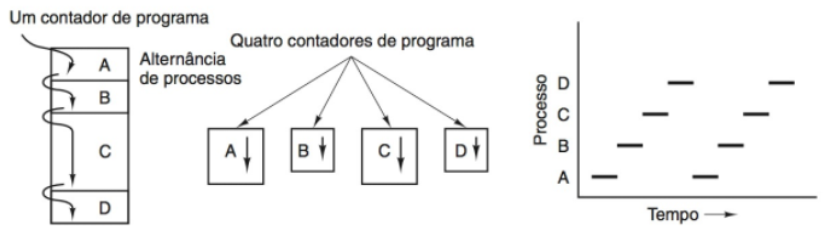
\includegraphics[keepaspectratio, width=.9\textwidth]{../figs/cap03/multiprog.png}
	\end{figure}
	
	\end{frame}

	\section{Processo}	
	
	\begin{frame}{Programa x Processo}
		\begin{itemize}
			\item Programa
			\begin{itemize}
				\item Conjunto de instruções para realizar uma tarefa
				\item Entidade passiva
			\end{itemize}
			\vspace{1em}
			\item Processo
			\begin{itemize}
				\item Entidade ativa
				\item Contém informações sobre a execução
			\end{itemize}
		\end{itemize}
	\end{frame}	
	
	\begin{frame}{Estrutura do processo}	
		\begin{figure}[hbtp]
		\centering
		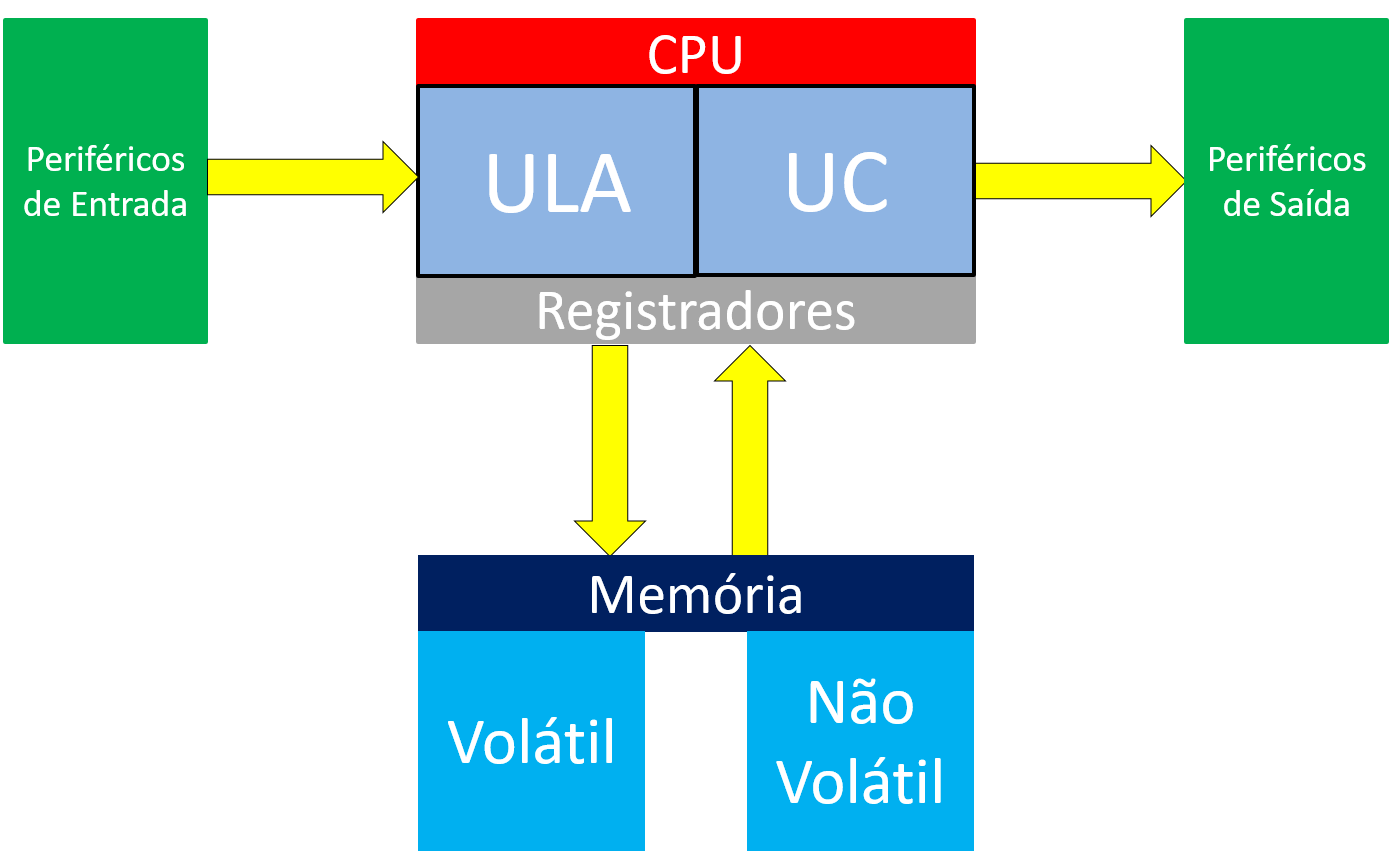
\includegraphics[keepaspectratio, height=.8\textheight]{../figs/cap03/estrutura.png}
		\end{figure}
	\end{frame}	
	
	\begin{frame}{Contexto de hardware}
		\begin{figure}[hbtp]
			\centering
			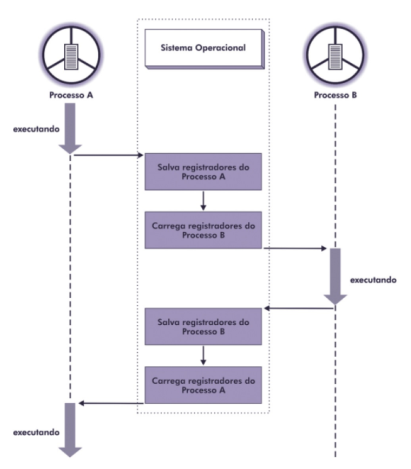
\includegraphics[keepaspectratio, height=.8\textheight]{../figs/cap03/contextohard.png}
		\end{figure}
	\end{frame}
	
	\begin{frame}{Contexto de software}
		\begin{itemize}
			\item Especificação de limites e  características dos recursos que podem ser alocados pelo processo
			\vspace{1em}
			\item Arquivo de usuários
			\begin{itemize}
				\item Especificação dos limites de recursos que cada processo pode alocar		
			\end{itemize}
			\vspace{1em}
			\item Grupos de informação
			\begin{itemize}
				\item Identificação
				\item Quotas 
				\item Privilégios
			\end{itemize}
		\end{itemize}
	\end{frame}
	
	\begin{frame}{Identificação}
		\begin{itemize}
			\item PID - \textit{Process Identification}
			\begin{itemize}
				\item Número único para o processo
				\item Pode ser utilizado por outros processos para comunicação
			\end{itemize}
			\vspace{1em}
			\item UID - \textit{User Identification}
			\begin{itemize}
				\item Identifica o usuário ou processo criador 
				\item Segurança
			\end{itemize}
		\end{itemize}
	\end{frame}
	
	\begin{frame}{Quotas}
		\begin{itemize}
			\item Limites de cada recurso do sistema que um processo pode alocar
			\begin{itemize}
				\item número máximo de arquivos abertos simultaneamente; 
				\item tamanho máximo de memória principal e secundária que o processo pode alocar; 
				\item número máximo de operações de E/S pendentes; 
				\item tamanho máximo do buffer para operações de E/S; 
				\item número máximo de processos, subprocessos e threads que podem ser criados
			\end{itemize}
		\end{itemize}
	\end{frame}
	
	\begin{frame}{Privilégios}
		\begin{itemize}
			\item  Definem as ações que um processo pode fazer em relação a ele
mesmo, aos demais processos e ao sistema operacional.
			\vspace{1em}
			\item Privilégios que afetam processos
			\begin{itemize}
				\item Prioridade de execução
				\item Limites de alocação de memória
			\end{itemize}
			\vspace{1em}
			\item Privilégios que afetam o sistema
			\begin{itemize}
				\item Operação e gerência do sistema
				\item Conta de acesso específica
			\end{itemize}
		\end{itemize}
	\end{frame}
	
	\begin{frame}{Espaço de endereçamento}
		\begin{itemize}
			\item Área de memória pertencente ao processo onde instruções e dados do programa são armazenados para execução.
			\vspace{1em}
			\item Exclusivo para cada processo
		\end{itemize}
	\end{frame}
	
	\begin{frame}{Estrutura do processo}	
		\begin{figure}[hbtp]
			\centering
			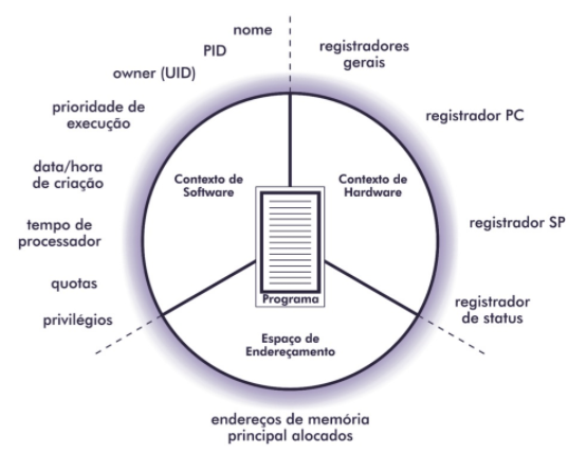
\includegraphics[keepaspectratio, height=.8\textheight]{../figs/cap03/estrutura1.png}
		\end{figure}
	\end{frame}	
	
	\begin{frame}{Bloco de Controle do Processo - BCP}
		\begin{itemize}
			\item Estrutura de dados responsável pela implementação do processo pelo sistema operacional
			\vspace{1em}
			\item Mantém informações sobre o contexto de hardware, contexto de software e espaço de endereçamento de cada processo
			\vspace{1em}
			\item Armazenados em área exclusiva na memória principal
			\begin{itemize}
				\item Tamanho da área pode ser configurado no sistema operacional
			\end{itemize}
		\end{itemize}
	\end{frame}
	
	\begin{frame}{Composição do BCP}
		\begin{itemize}
			\item Identificador da tarefa
				\vspace{1em}
			\item Estado da tarefa
				\vspace{1em}
			\item Informações de contexto do processador
				\vspace{1em}
			\item Lista de recursos utilizados (arquivos abertos, conexões de rede)
				\vspace{1em}
			\item Informações de gerência e contabilização
		\end{itemize}
	\end{frame}
	
	\begin{frame}{Trocas de contexto}
		 \begin{itemize}
		 	\item Ato de salvar os valores de contexto de um processo e restaurar o contexto de outro processo
		 	\vspace{1em}
		 	\item Codificada em linguagem de máquina
		 	\vspace{1em}
		 	\item \textit{Dispatcher}
		 	\begin{itemize}
		 		\item Responsável pelo armazenamento e recuperação do contexto
		 	\end{itemize}
		 	\vspace{1em}
		 	\item Escalonador (\textit{scheduler})
		 	\begin{itemize}
		 		\item Decide qual processo será o próximo a ser executado
		 	\end{itemize}
		 \end{itemize}
	\end{frame}

	\section{Estados do Processo}	
	
	\begin{frame}{Estados do processo}
		\begin{itemize}
			\item Novo
			\begin{itemize}
				\item O processo está em fase de criação
			\end{itemize}
			\vspace{0.75em}
			\item Em execução
			\begin{itemize}
				\item Instruções sendo executadas
			\end{itemize}
			\vspace{0.75em}
			\item Em espera (bloqueado)
			\begin{itemize}
				\item O processo está esperando que algum evento ocorra 
			\end{itemize}
			\vspace{0.75em}
			\item Pronto
			\begin{itemize}
				\item O processo está esperando que seja atribuído a um processador
			\end{itemize}
			\vspace{0.75em}
			\item Concluído
			\begin{itemize}
				\item O processo terminou sua execução.
			\end{itemize}
		\end{itemize}
	\end{frame}
	
	\begin{frame}{Transições de estado}
		
	\begin{figure}[hbtp]
	\centering
	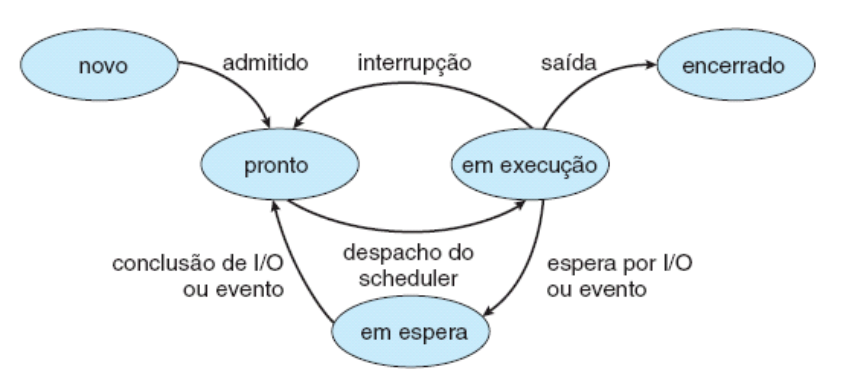
\includegraphics[keepaspectratio, width=.9\textwidth]{../figs/cap03/estados.png}	
	\end{figure}
	\end{frame}	
	
	\begin{frame}{Criação de processos}
		\begin{itemize}
			\item Sistemas de propósito específico
			\begin{itemize}
				\item Possível iniciar todos os processos necessários quando o sistema inicia
			\end{itemize}
			\vspace{1em}
			\item Sistemas de propósito geral 
			\begin{itemize}
				\item Criação e encerramento de processos durante a operação
			\end{itemize}
		\end{itemize}
	\end{frame}
	

	\begin{frame}{Eventos de criação de processos}
		\begin{itemize}
			\item Inicialização do sistema. 
			\vspace{1em}
			\item Realização de uma chamada de sistema por um processo em execução para criação de processo.
			\vspace{1em} 
			\item Um pedido de usuário para criar um novo processo. 
			\vspace{1em}
			\item Início de uma tarefa em lote.
		\end{itemize}
	\end{frame}
	
	\begin{frame}{Condições de término de processos}
		\begin{itemize}
			\item Término normal (voluntário) 
			\vspace{1em}
			\item Término por erro (voluntário) 
			\vspace{1em}
			\item Erro fatal (involuntário) 
			\vspace{1em}
			\item Eliminado por outro processo (involuntário)
		\end{itemize}
	\end{frame}

	\begin{frame}{CPU-Bound x I/O-bound}
	\begin{itemize}
		\item CPU-bound
		\begin{itemize}
			\item Processo que passa a maior parte do tempo em estado de execução	
		\end{itemize}
		\item I/O-bound
		\begin{itemize}
			\item Processo que passa a maior parte do tempo em estado de espera	
		\end{itemize}
		
	\end{itemize}
	\end{frame}
	
	\begin{frame}{Foreground x Background}
		\begin{itemize}
			\item \textit{Foreground}
			\begin{itemize}
				\item Permite comunicação direta do usuário com o processo
			\end{itemize}
			\item \textit{Background}
			\begin{itemize}
				\item Não existe comunicação do processo com o usuário 
			\end{itemize}
		\end{itemize}
	\end{frame}
	
	\begin{frame}
		\frametitle{Bibliografia}
		\begin{itemize}
			\item SILBERSCHATZ, A.; GALVIN, P. B.; GAGNE, G.. \textbf{Fundamentos de sistmas operacionais: princípios básicos.} Rio de Janeiro: LTC – Livros Técnicos e Científicos, 2013.
			
			\vspace{1em}

			\item TANENBAUM, A.S., WOODHULL, A.S. \textbf{Sistemas Operacionais.} Porto Alegre: Grupo A, 2008.
			
			\vspace{1em}
			
			\item MACHADO, F.B.; MAIA, L.P. \textbf{Fundamentos de Sistemas Operacionais.} Porto Alegre: Grupo GEN, 2011.
		\end{itemize}
	\end{frame}


	\begin{frame}{}
	\end{frame}	
	
\end{document}
